% Options for packages loaded elsewhere
% Options for packages loaded elsewhere
\PassOptionsToPackage{unicode}{hyperref}
\PassOptionsToPackage{hyphens}{url}
%
\documentclass[
  ignorenonframetext,
  aspectratio=169,
  russian,
]{beamer}
\newif\ifbibliography
\usepackage{pgfpages}
\setbeamertemplate{caption}[numbered]
\setbeamertemplate{caption label separator}{: }
\setbeamercolor{caption name}{fg=normal text.fg}
\beamertemplatenavigationsymbolshorizontal
% Prevent slide breaks in the middle of a paragraph
\widowpenalties 1 10000
\raggedbottom
\AtBeginPart{
  \frame{\partpage}
}
\AtBeginSection{
  \ifbibliography
  \else
    \frame{\sectionpage}
  \fi
}
\AtBeginSubsection{
  \frame{\subsectionpage}
}
\usepackage{iftex}
\ifPDFTeX
  \usepackage[T1]{fontenc}
  \usepackage[utf8]{inputenc}
  \usepackage{textcomp} % provide euro and other symbols
\else % if luatex or xetex
  \usepackage{unicode-math} % this also loads fontspec
  \defaultfontfeatures{Scale=MatchLowercase}
  \defaultfontfeatures[\rmfamily]{Ligatures=TeX,Scale=1}
\fi
\usepackage{lmodern}

\usetheme[]{Montpellier}
\usecolortheme[]{seagull}
\ifPDFTeX\else
  % xetex/luatex font selection
\fi
% Use upquote if available, for straight quotes in verbatim environments
\IfFileExists{upquote.sty}{\usepackage{upquote}}{}
\IfFileExists{microtype.sty}{% use microtype if available
  \usepackage[]{microtype}
  \UseMicrotypeSet[protrusion]{basicmath} % disable protrusion for tt fonts
}{}


\usepackage{longtable,booktabs,array}
\usepackage{calc} % for calculating minipage widths
\usepackage{caption}
% Make caption package work with longtable
\makeatletter
\def\fnum@table{\tablename~\thetable}
\makeatother
\usepackage{graphicx}
\makeatletter
\newsavebox\pandoc@box
\newcommand*\pandocbounded[1]{% scales image to fit in text height/width
  \sbox\pandoc@box{#1}%
  \Gscale@div\@tempa{\textheight}{\dimexpr\ht\pandoc@box+\dp\pandoc@box\relax}%
  \Gscale@div\@tempb{\linewidth}{\wd\pandoc@box}%
  \ifdim\@tempb\p@<\@tempa\p@\let\@tempa\@tempb\fi% select the smaller of both
  \ifdim\@tempa\p@<\p@\scalebox{\@tempa}{\usebox\pandoc@box}%
  \else\usebox{\pandoc@box}%
  \fi%
}
% Set default figure placement to htbp
\def\fps@figure{htbp}
\makeatother



\ifLuaTeX
\usepackage[bidi=basic,provide=*]{babel}
\else
\usepackage[bidi=default,provide=*]{babel}
\fi
% get rid of language-specific shorthands (see #6817):
\let\LanguageShortHands\languageshorthands
\def\languageshorthands#1{}


\setlength{\emergencystretch}{3em} % prevent overfull lines

\providecommand{\tightlist}{%
  \setlength{\itemsep}{0pt}\setlength{\parskip}{0pt}}



 

\usepackage[]{csquotes}

\usepackage{libertine}
\makeatletter
\@ifpackageloaded{caption}{}{\usepackage{caption}}
\AtBeginDocument{%
\ifdefined\contentsname
  \renewcommand*\contentsname{Содержание}
\else
  \newcommand\contentsname{Содержание}
\fi
\ifdefined\listfigurename
  \renewcommand*\listfigurename{Список иллюстраций}
\else
  \newcommand\listfigurename{Список иллюстраций}
\fi
\ifdefined\listtablename
  \renewcommand*\listtablename{Список таблиц}
\else
  \newcommand\listtablename{Список таблиц}
\fi
\ifdefined\figurename
  \renewcommand*\figurename{Рисунок}
\else
  \newcommand\figurename{Рисунок}
\fi
\ifdefined\tablename
  \renewcommand*\tablename{Таблица}
\else
  \newcommand\tablename{Таблица}
\fi
}
\@ifpackageloaded{float}{}{\usepackage{float}}
\floatstyle{ruled}
\@ifundefined{c@chapter}{\newfloat{codelisting}{h}{lop}}{\newfloat{codelisting}{h}{lop}[chapter]}
\floatname{codelisting}{Список}
\newcommand*\listoflistings{\listof{codelisting}{Листинги}}
\makeatother
\makeatletter
\makeatother
\makeatletter
\@ifpackageloaded{caption}{}{\usepackage{caption}}
\@ifpackageloaded{subcaption}{}{\usepackage{subcaption}}
\makeatother

\usepackage{bookmark}
\IfFileExists{xurl.sty}{\usepackage{xurl}}{} % add URL line breaks if available
\urlstyle{same}
\hypersetup{
  pdftitle={Лабораторная работа},
  pdfauthor={Андрюшин Никита Сергеевич},
  pdflang={ru-RU},
  hidelinks,
  pdfcreator={LaTeX via pandoc}}


\title{Лабораторная работа}
\subtitle{Презентация 1}
\author{Андрюшин Никита Сергеевич}
\date{2025-09-13}

\begin{document}
\frame{\titlepage}

\renewcommand*\contentsname{Содержание}
\begin{frame}[allowframebreaks]
  \frametitle{Содержание}
  \setcounter{tocdepth}{2}
  \tableofcontents
\end{frame}
\setcounter{tocdepth}{2}
\tableofcontents
}

\section{1. Информация}\label{ux438ux43dux444ux43eux440ux43cux430ux446ux438ux44f}

\begin{frame}{1.1 Докладчик}
\phantomsection\label{ux434ux43eux43aux43bux430ux434ux447ux438ux43a}
\begin{columns}[c]
\begin{column}{0.7\linewidth}
\begin{itemize}[<+->]
\tightlist
\item
  Андрюшин Никита Сергеевич
\item
  Российский университет дружбы народов им. П. Лумумбы
\end{itemize}
\end{column}

\begin{column}{0.3\linewidth}
\pandocbounded{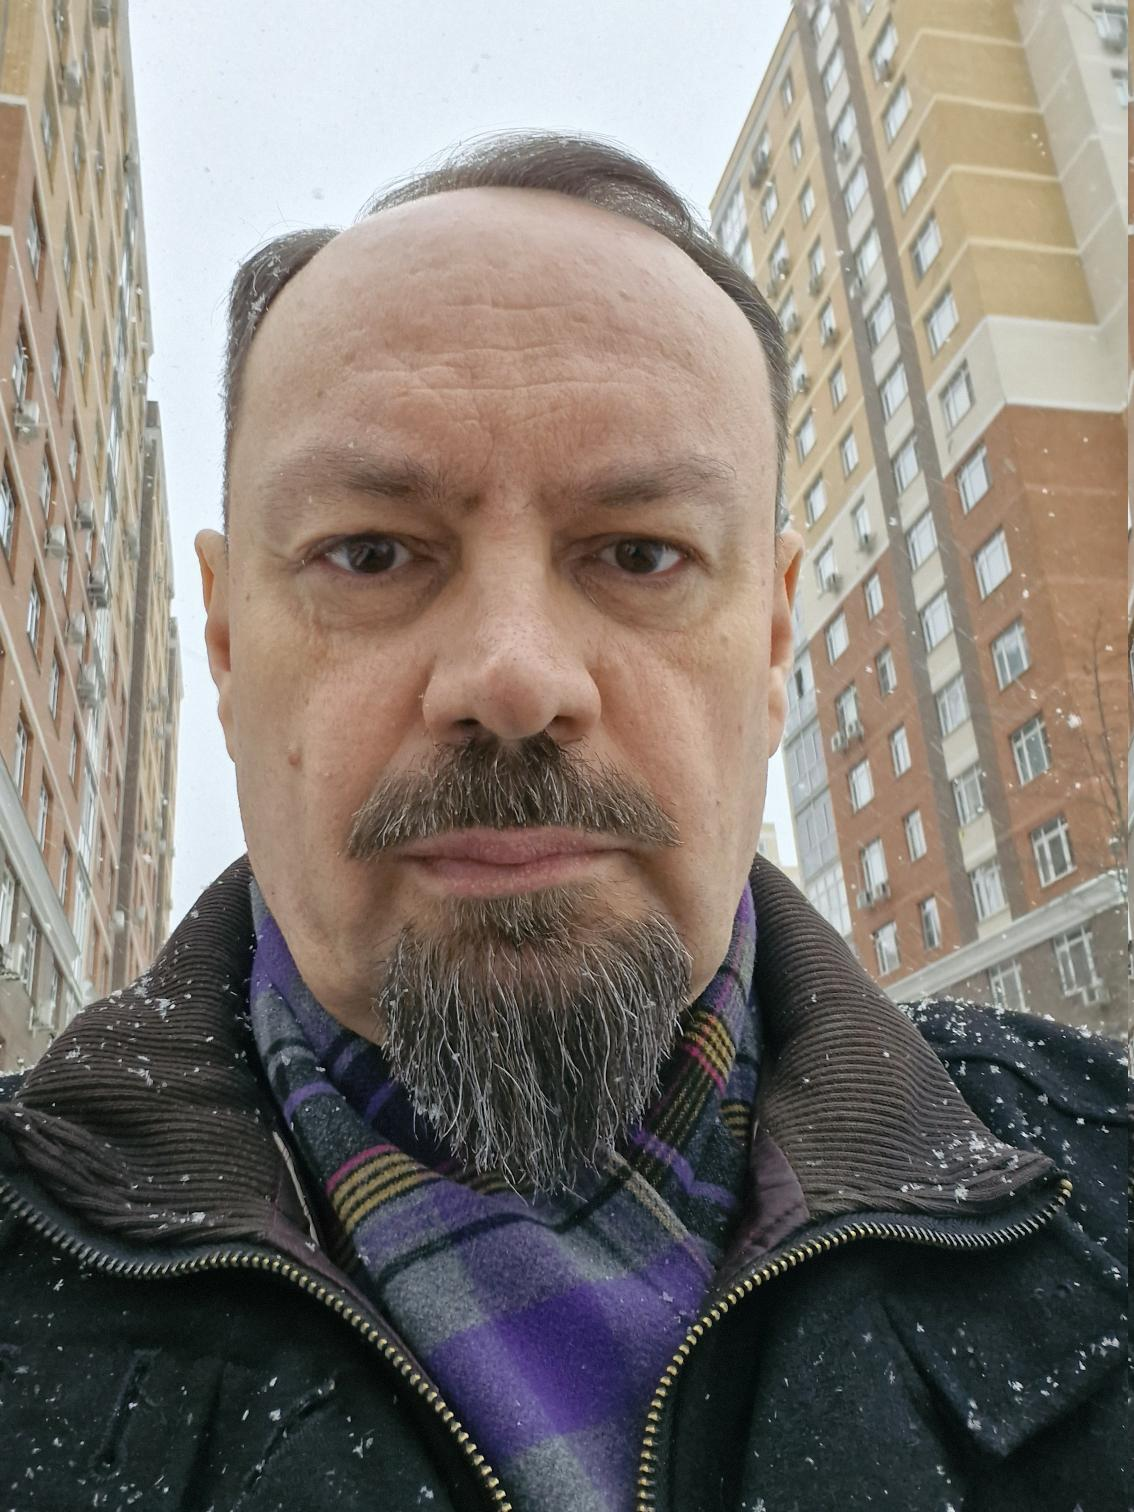
\includegraphics[keepaspectratio]{./image/kulyabov.jpg}}
\end{column}
\end{columns}
\end{frame}

\begin{frame}{1.2 Цель}
\phantomsection\label{ux446ux435ux43bux44c}
Приобретение практических навыков по установке и конфигурированию
DNS-сервера, усвоение принципов работы системы доменных имён.
\end{frame}

\begin{frame}{1.3 Запуск ВМ}
\phantomsection\label{ux437ux430ux43fux443ux441ux43a-ux432ux43c}
Для начала запустим виртуальную машину через vagrant

\begin{figure}[H]

{\centering \pandocbounded{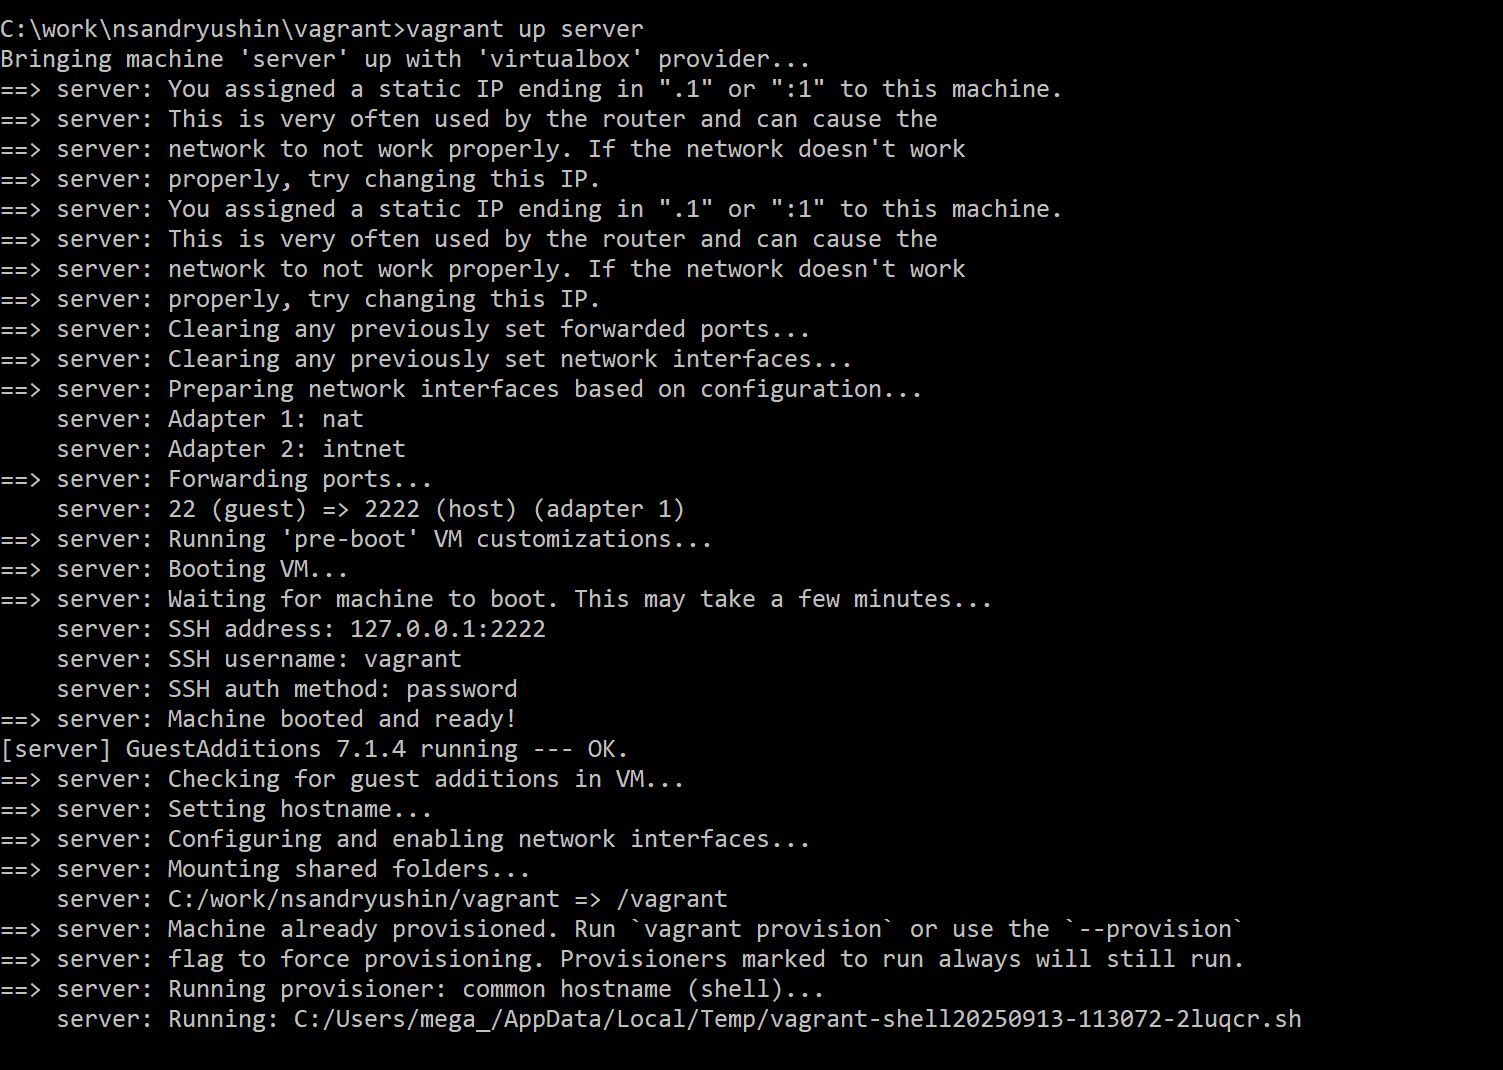
\includegraphics[keepaspectratio]{image/1.png}}

}

\caption{Запуск ВМ}

\end{figure}%
\end{frame}

\begin{frame}{1.4 Скачивание пакетов}
\phantomsection\label{ux441ux43aux430ux447ux438ux432ux430ux43dux438ux435-ux43fux430ux43aux435ux442ux43eux432}
Теперь скачаем пакет bind utils

\begin{figure}[H]

{\centering \pandocbounded{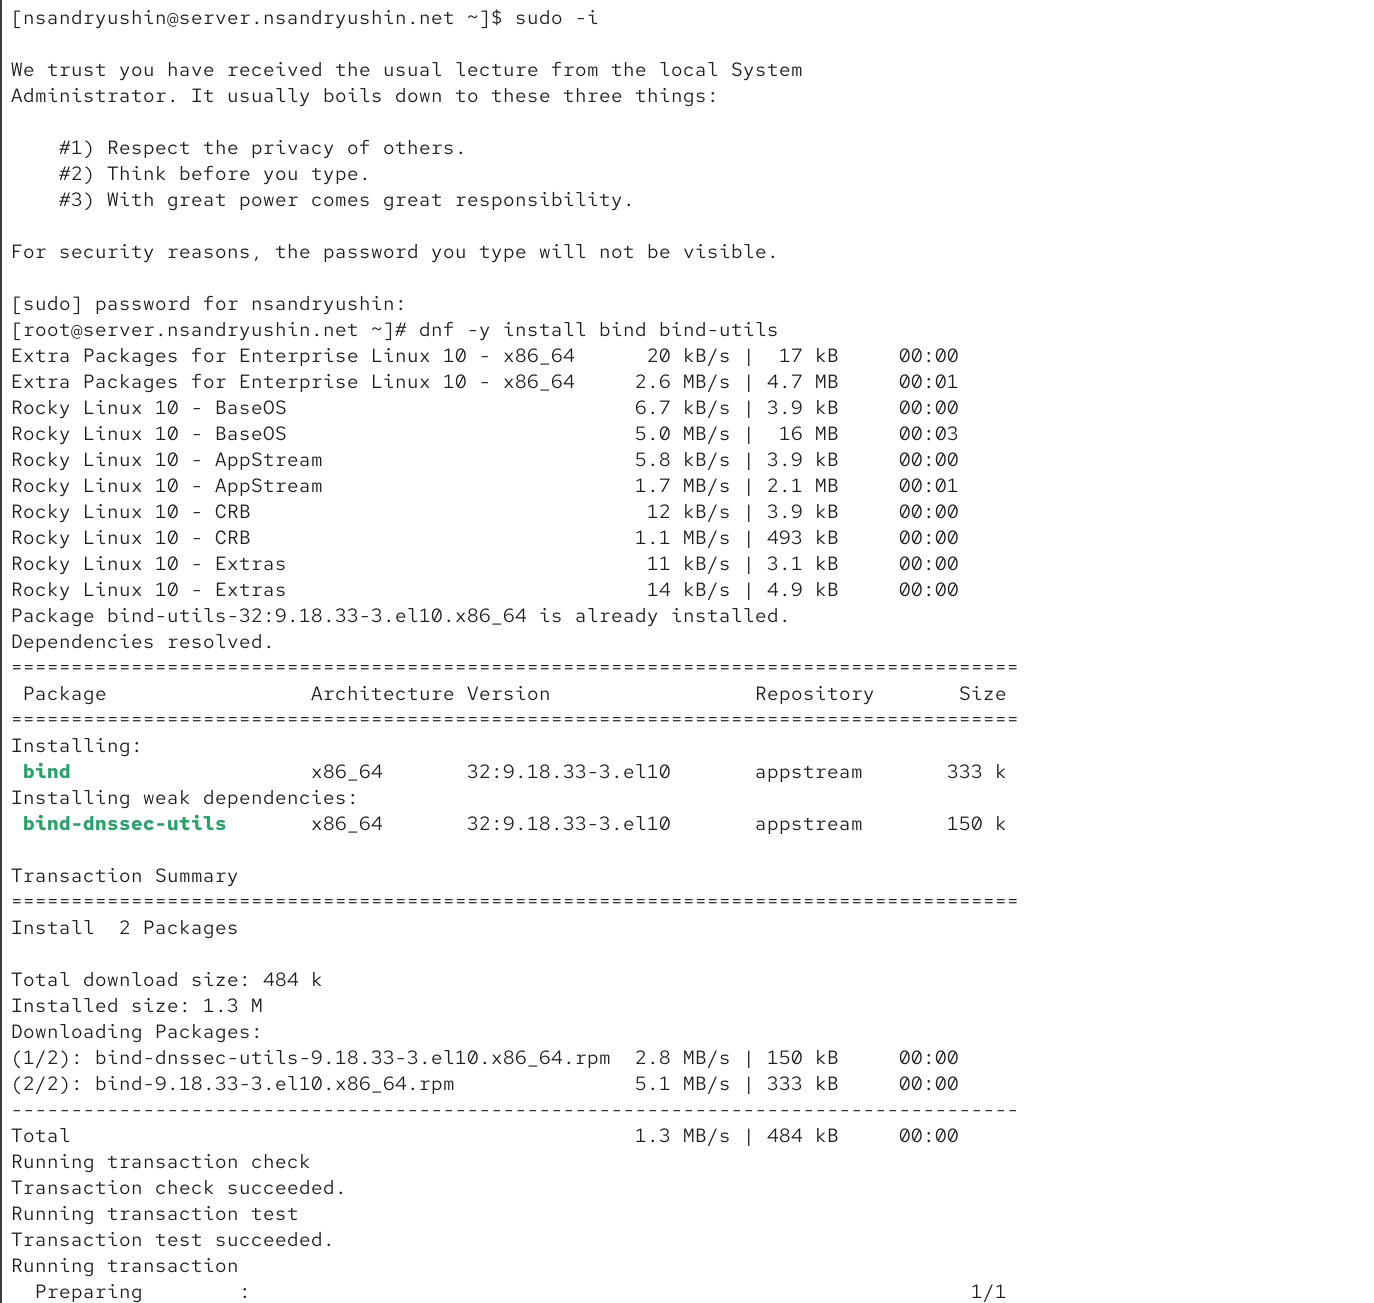
\includegraphics[keepaspectratio]{image/2.png}}

}

\caption{Скачивание пакетов}

\end{figure}%
\end{frame}

\begin{frame}{1.5 dig ya.ru}
\phantomsection\label{dig-ya.ru}
Используем команду dig для проверки сервисов яндекса

\begin{figure}[H]

{\centering \pandocbounded{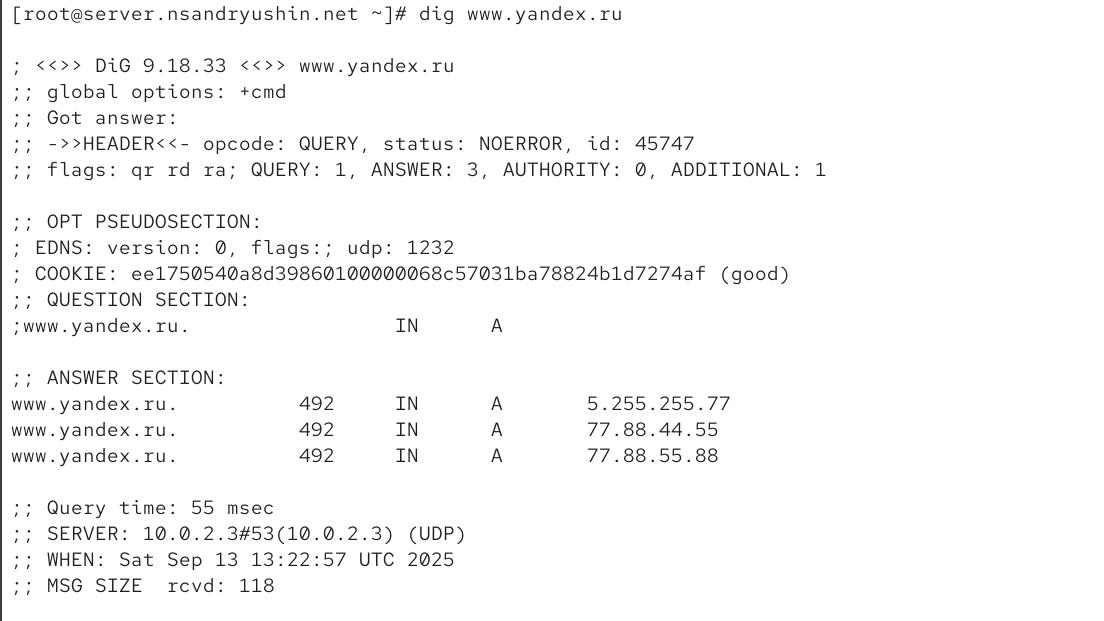
\includegraphics[keepaspectratio]{image/3.png}}

}

\caption{dig ya.ru}

\end{figure}%
\end{frame}

\begin{frame}{1.6 Файлы конфигурации}
\phantomsection\label{ux444ux430ux439ux43bux44b-ux43aux43eux43dux444ux438ux433ux443ux440ux430ux446ux438ux438}
Посморим на содержание файлов конфигурации dns в etc

\begin{figure}[H]

{\centering \pandocbounded{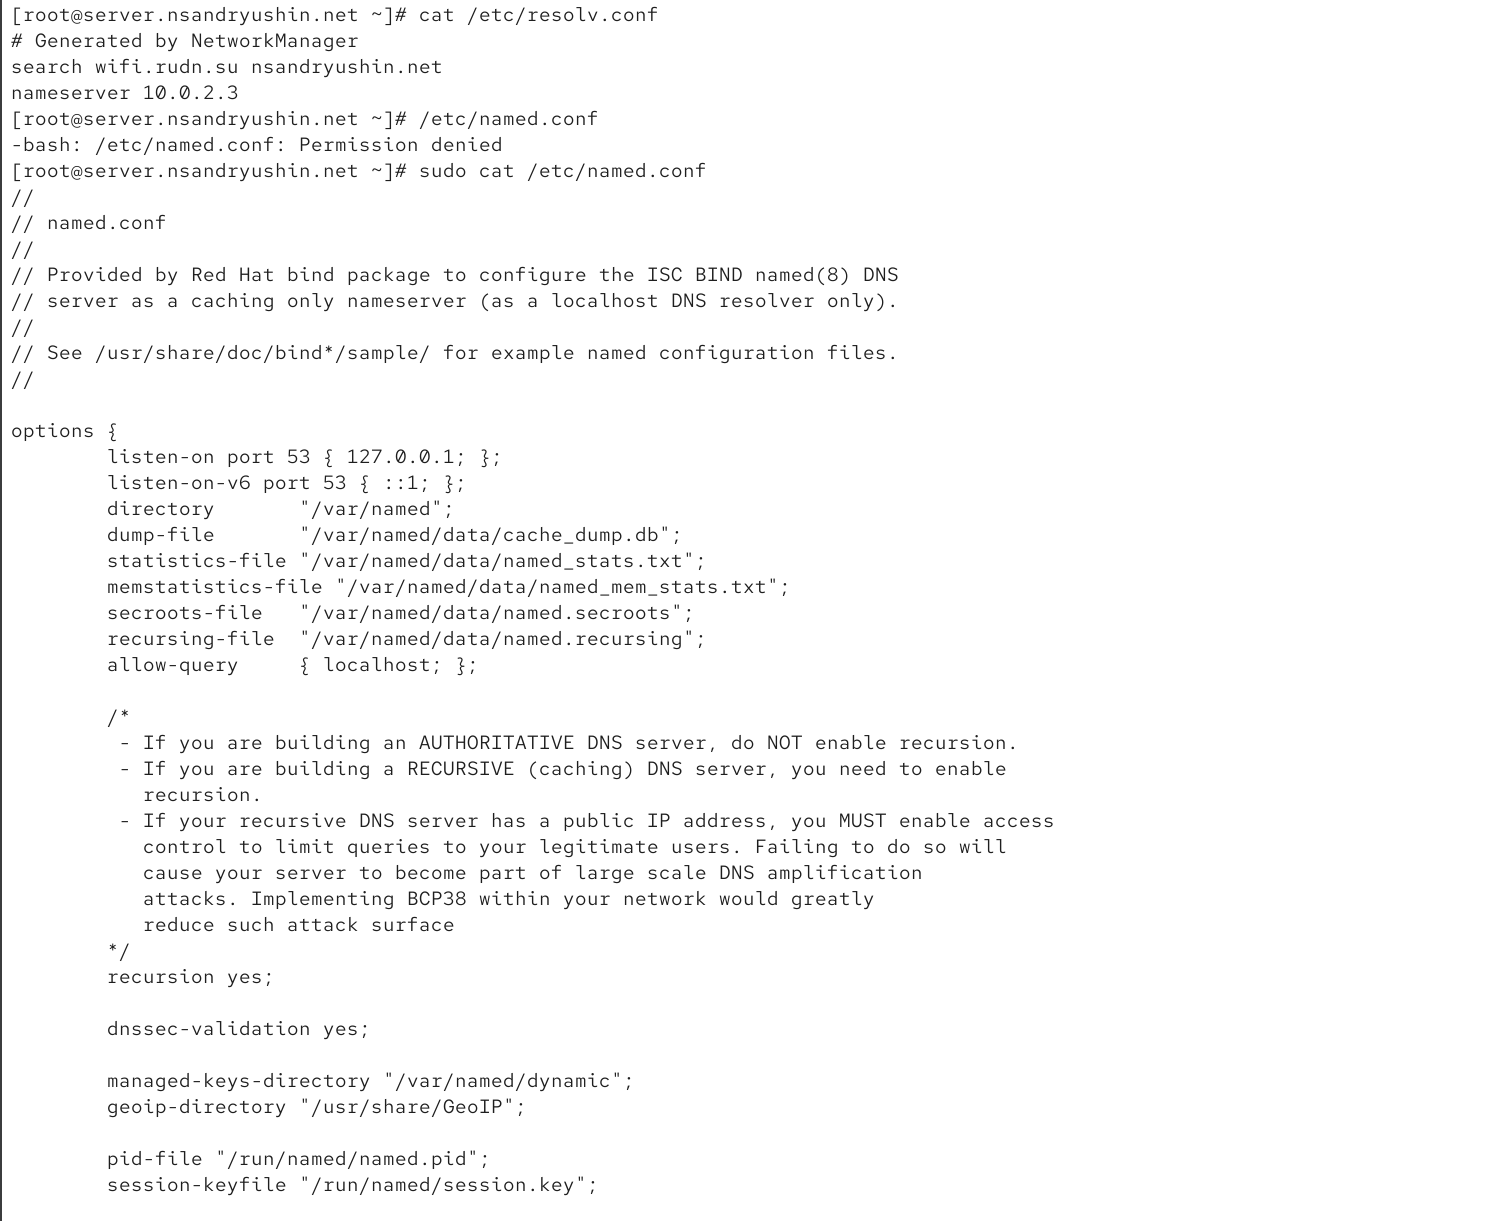
\includegraphics[keepaspectratio]{image/4.png}}

}

\caption{Файлы конфигурации}

\end{figure}%
\end{frame}

\begin{frame}{1.7 named.ca}
\phantomsection\label{named.ca}
Просморим теперь файл named.ca

\begin{figure}[H]

{\centering \pandocbounded{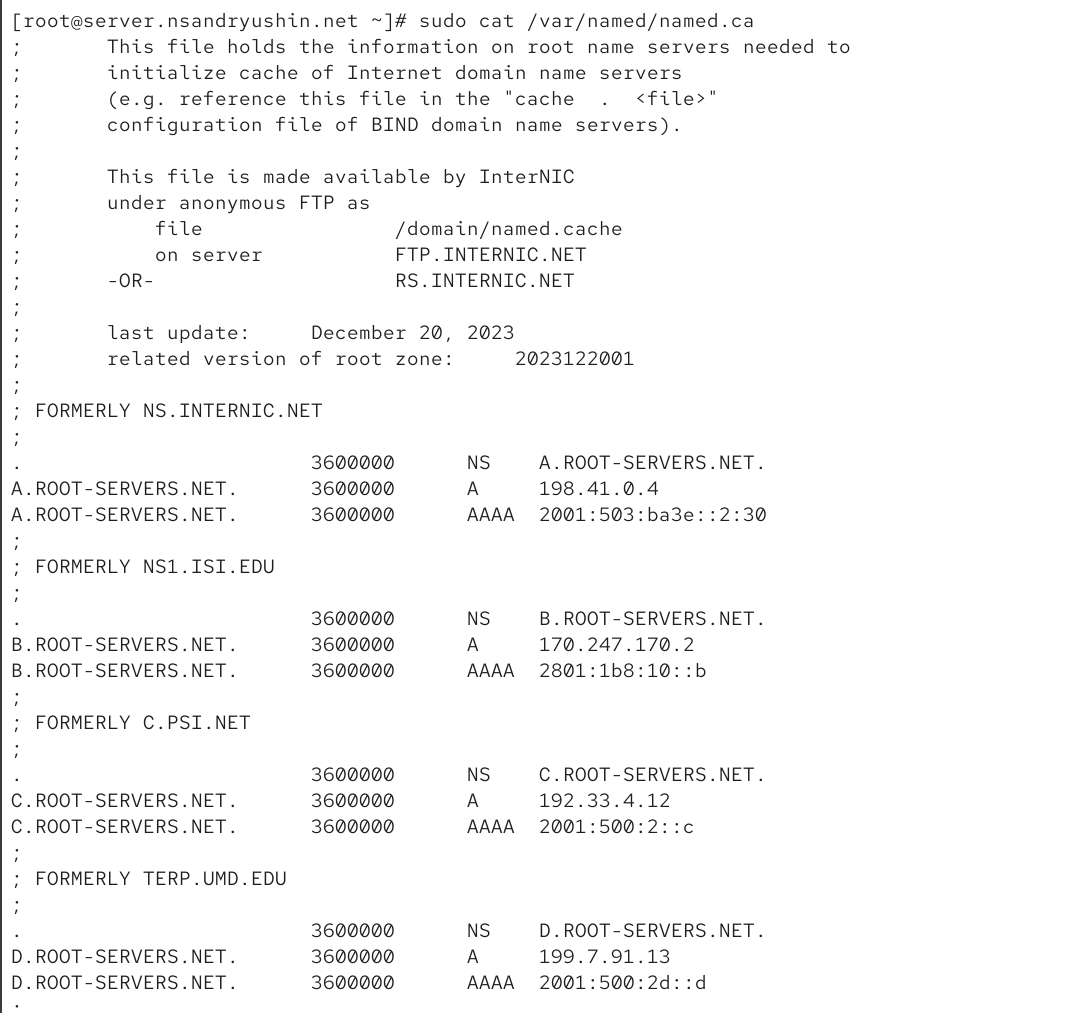
\includegraphics[keepaspectratio]{image/5.png}}

}

\caption{named.ca}

\end{figure}%
\end{frame}

\begin{frame}{1.8 named.localhost и named.loopback}
\phantomsection\label{named.localhost-ux438-named.loopback}
Содержимое named.localhost и named.loopback

\begin{figure}[H]

{\centering \pandocbounded{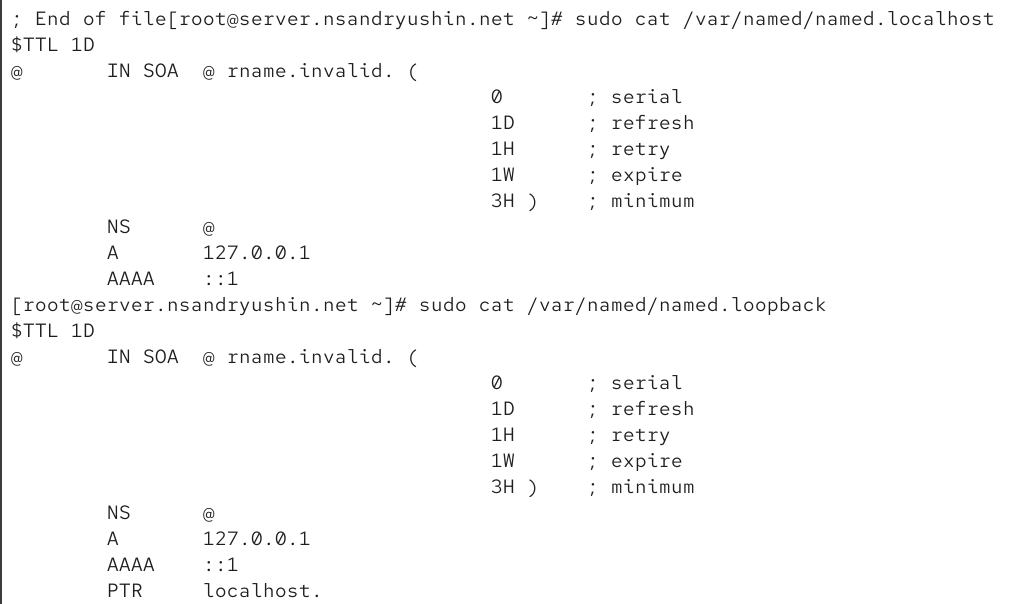
\includegraphics[keepaspectratio]{image/6.png}}

}

\caption{named.localhost и named.loopback}

\end{figure}%
\end{frame}

\begin{frame}{1.9 Запуск named}
\phantomsection\label{ux437ux430ux43fux443ux441ux43a-named}
Запустим теперь named и осуществим снова dig yandex.ru

\begin{figure}[H]

{\centering \pandocbounded{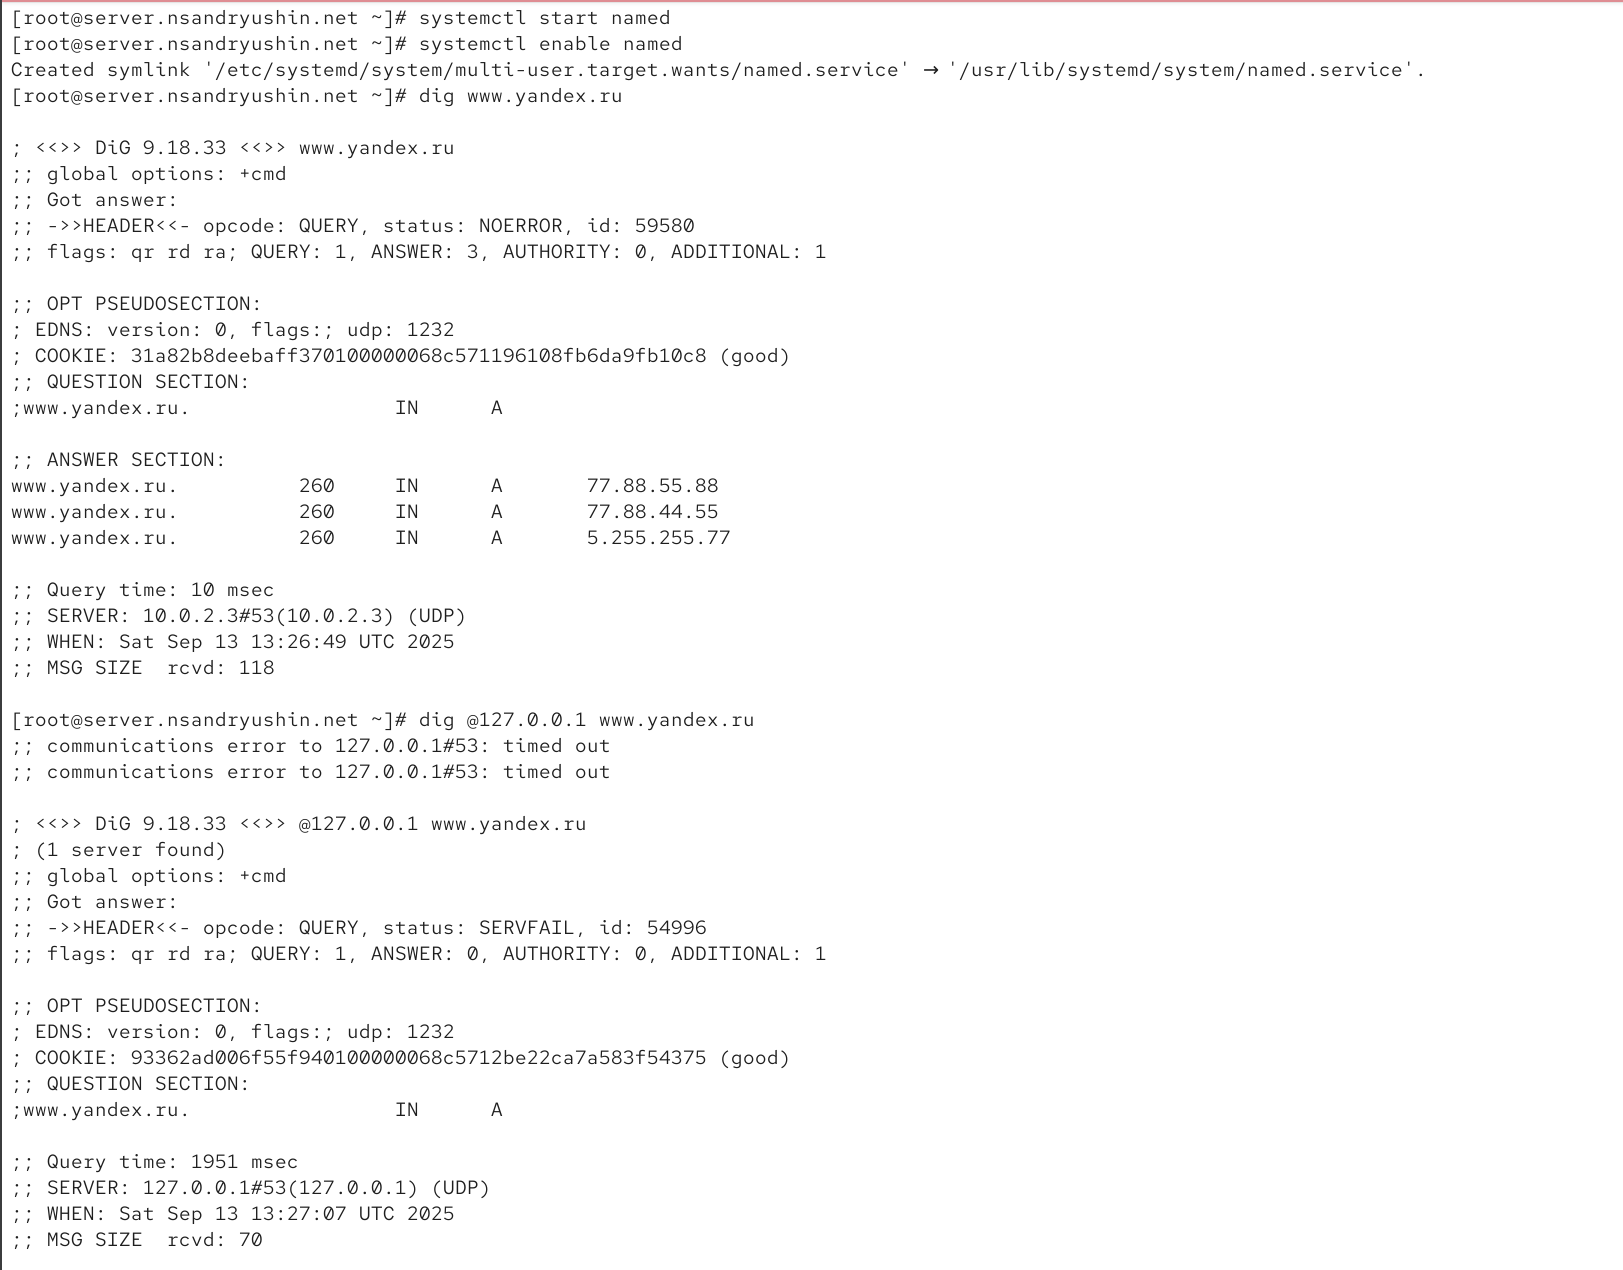
\includegraphics[keepaspectratio]{image/7.png}}

}

\caption{Запуск named}

\end{figure}%
\end{frame}

\begin{frame}{1.10 eth0}
\phantomsection\label{eth0}
Теперь настроим порт eth0

\begin{figure}[H]

{\centering \pandocbounded{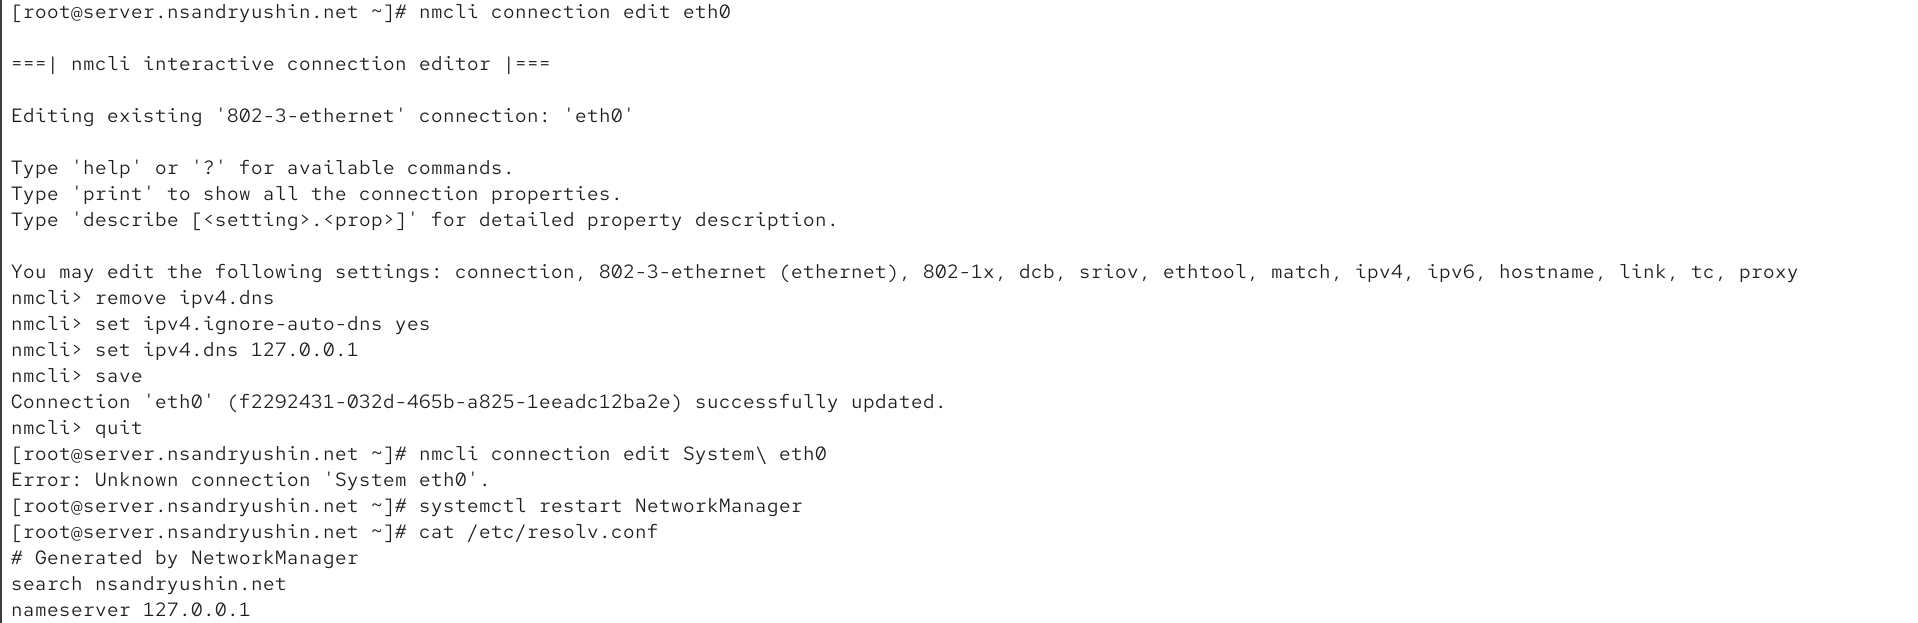
\includegraphics[keepaspectratio]{image/8.png}}

}

\caption{eth0}

\end{figure}%
\end{frame}

\begin{frame}{1.11 named.conf}
\phantomsection\label{named.conf}
Откроем и отредактируем named.conf

\begin{figure}[H]

{\centering \pandocbounded{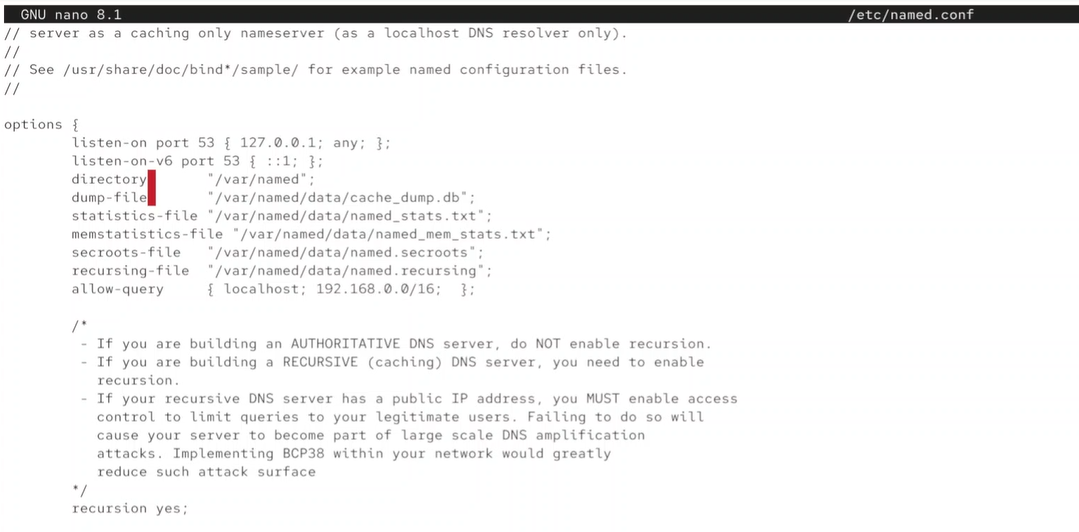
\includegraphics[keepaspectratio]{image/9.png}}

}

\caption{named.conf}

\end{figure}%
\end{frame}

\begin{frame}{1.12 Правила фаервола}
\phantomsection\label{ux43fux440ux430ux432ux438ux43bux430-ux444ux430ux435ux440ux432ux43eux43bux430}
Установим правила фаервола

\begin{figure}[H]

{\centering \pandocbounded{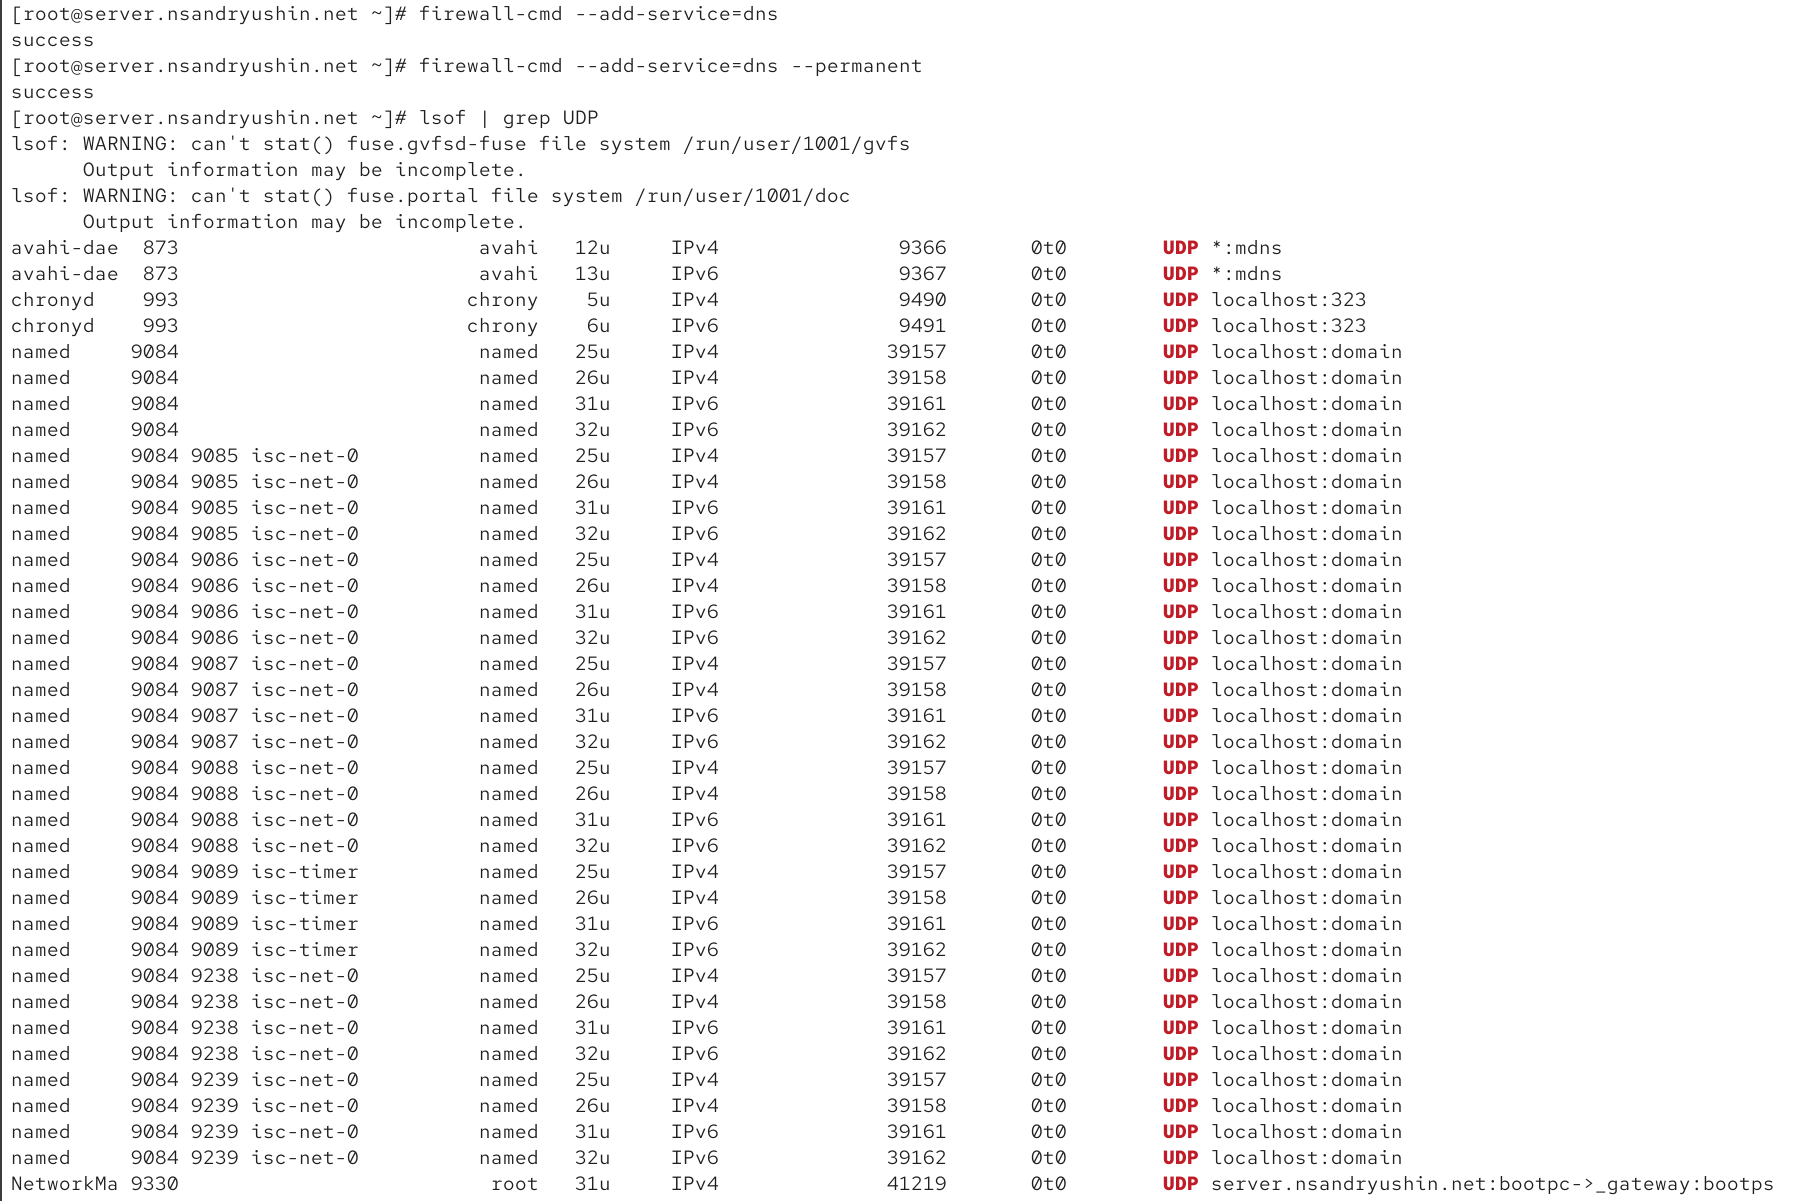
\includegraphics[keepaspectratio]{image/10.png}}

}

\caption{Правила фаервола}

\end{figure}%
\end{frame}

\begin{frame}{1.13 перемещение файла}
\phantomsection\label{ux43fux435ux440ux435ux43cux435ux449ux435ux43dux438ux435-ux444ux430ux439ux43bux430}
Теперь переместим файл с настройкой конфига

\begin{figure}[H]

{\centering \pandocbounded{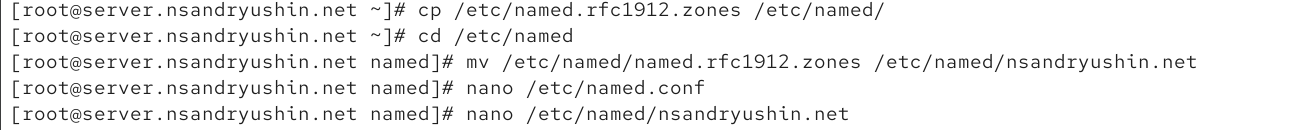
\includegraphics[keepaspectratio]{image/11.png}}

}

\caption{перемещение файла}

\end{figure}%
\end{frame}

\begin{frame}{1.14 Редактирование файла}
\phantomsection\label{ux440ux435ux434ux430ux43aux442ux438ux440ux43eux432ux430ux43dux438ux435-ux444ux430ux439ux43bux430}
И отредактируем наш файл под наши параметры

\begin{figure}[H]

{\centering \pandocbounded{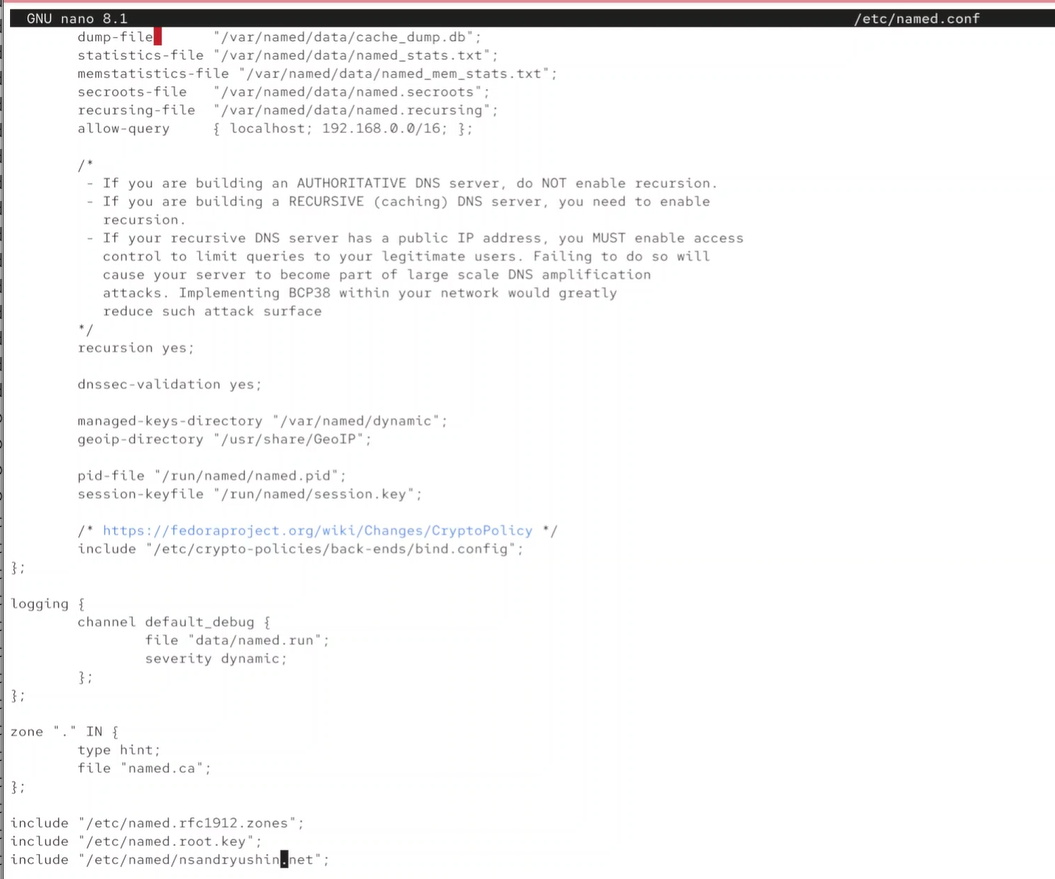
\includegraphics[keepaspectratio]{image/12.png}}

}

\caption{Редактирование файла}

\end{figure}%
\end{frame}

\begin{frame}{1.15 Файл зон}
\phantomsection\label{ux444ux430ux439ux43b-ux437ux43eux43d}
То же самое сделаем с файлом зон

\begin{figure}[H]

{\centering \pandocbounded{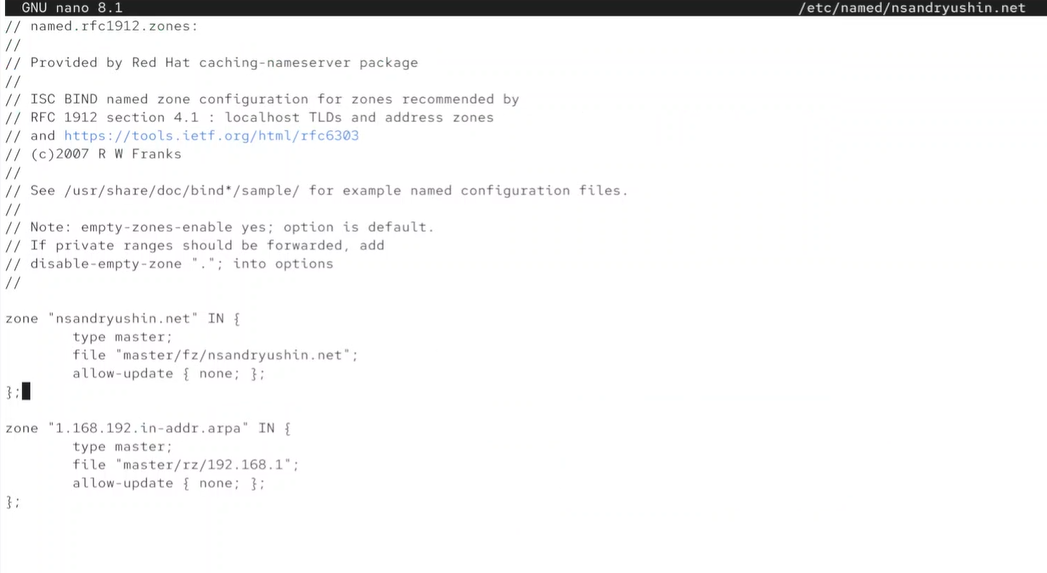
\includegraphics[keepaspectratio]{image/13.png}}

}

\caption{Файл зон}

\end{figure}%
\end{frame}

\begin{frame}{1.16 Создание папок и настроек днс}
\phantomsection\label{ux441ux43eux437ux434ux430ux43dux438ux435-ux43fux430ux43fux43eux43a-ux438-ux43dux430ux441ux442ux440ux43eux435ux43a-ux434ux43dux441}
Создадим папки с настройками днс

\begin{figure}[H]

{\centering \pandocbounded{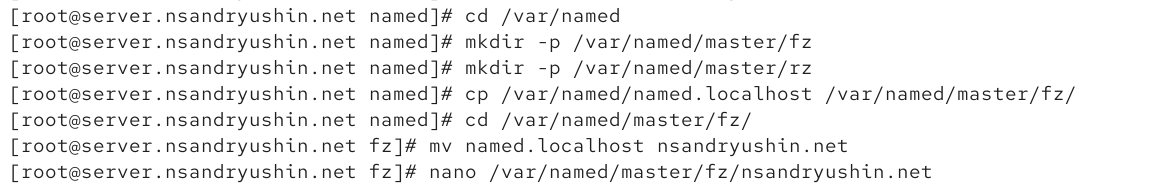
\includegraphics[keepaspectratio]{image/14.png}}

}

\caption{Создание папок и настроек днс}

\end{figure}%
\end{frame}

\begin{frame}{1.17 nsandryushin.net}
\phantomsection\label{nsandryushin.net}
Отредактируем файл nsandryushin.net

\begin{figure}[H]

{\centering \pandocbounded{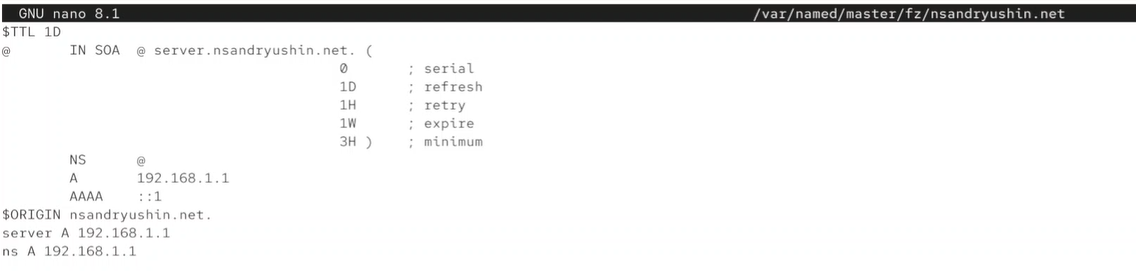
\includegraphics[keepaspectratio]{image/15.png}}

}

\caption{nsandryushin.net}

\end{figure}%
\end{frame}

\begin{frame}{1.18 Папка rz}
\phantomsection\label{ux43fux430ux43fux43aux430-rz}
Теперь посмотрим на файлы из папки rz

\begin{figure}[H]

{\centering \pandocbounded{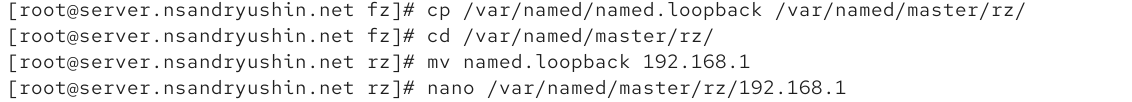
\includegraphics[keepaspectratio]{image/16.png}}

}

\caption{Папка rz}

\end{figure}%
\end{frame}

\begin{frame}{1.19 Редактирование файла}
\phantomsection\label{ux440ux435ux434ux430ux43aux442ux438ux440ux43eux432ux430ux43dux438ux435-ux444ux430ux439ux43bux430-1}
Отредактируем следующим образом

\begin{figure}[H]

{\centering \pandocbounded{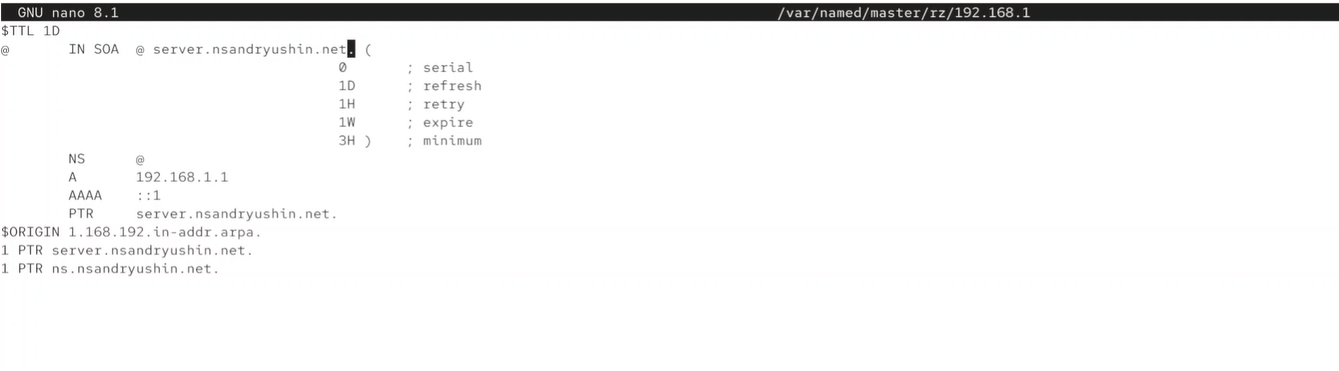
\includegraphics[keepaspectratio]{image/17.png}}

}

\caption{Редактирование файла}

\end{figure}%
\end{frame}

\begin{frame}{1.20 Selinux}
\phantomsection\label{selinux}
Настроим Selinux

\begin{figure}[H]

{\centering \pandocbounded{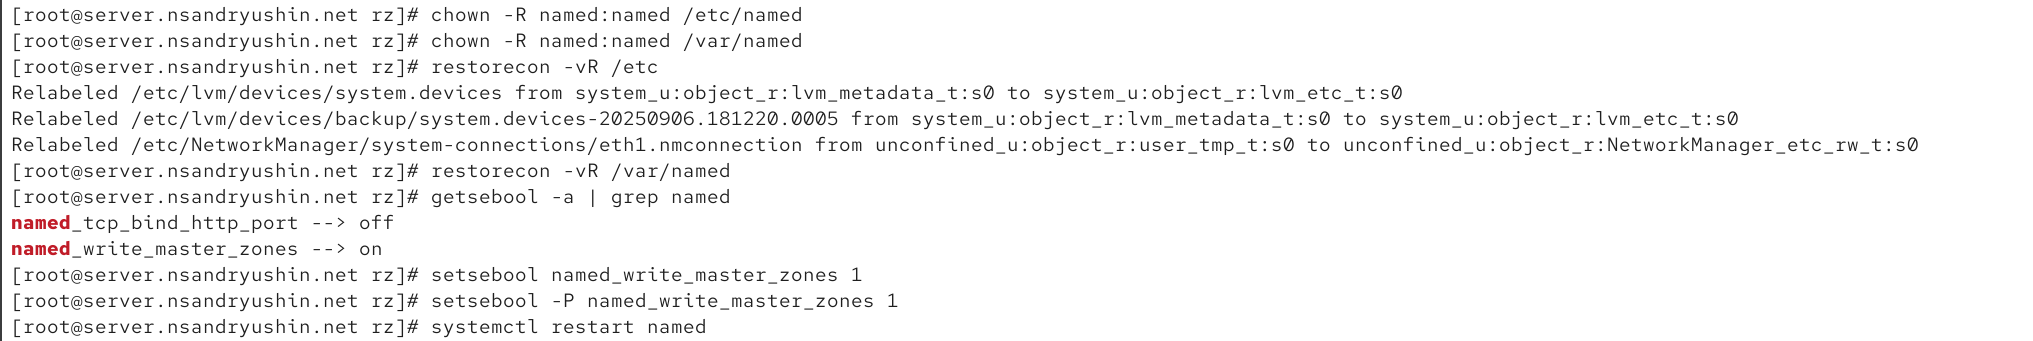
\includegraphics[keepaspectratio]{image/18.png}}

}

\caption{Selinux}

\end{figure}%
\end{frame}

\begin{frame}{1.21 dig}
\phantomsection\label{dig}
Через dig попробуем подключиться к собственному днс

\begin{figure}[H]

{\centering \pandocbounded{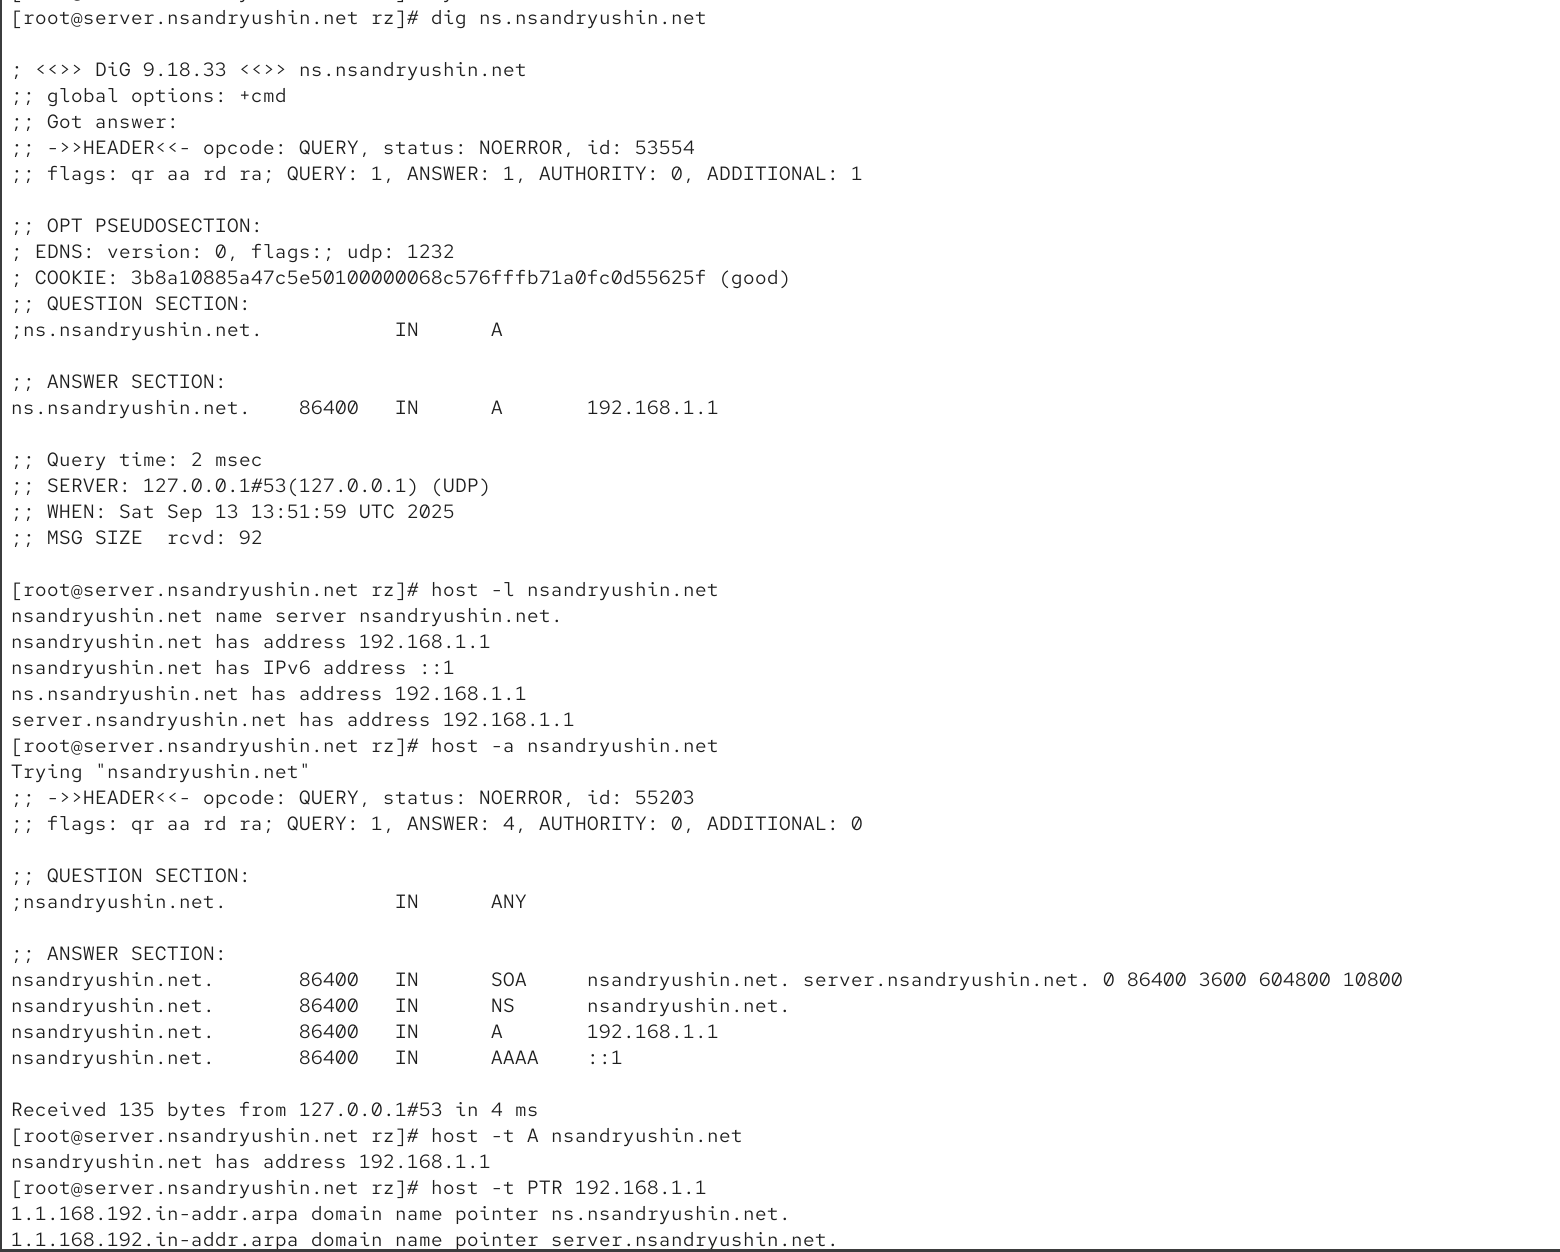
\includegraphics[keepaspectratio]{image/19.png}}

}

\caption{dig}

\end{figure}%
\end{frame}

\begin{frame}{1.22 Конфиг вагрант}
\phantomsection\label{ux43aux43eux43dux444ux438ux433-ux432ux430ux433ux440ux430ux43dux442}
Оформим нашу работу как конфигурацию для вагранта

\begin{figure}[H]

{\centering \pandocbounded{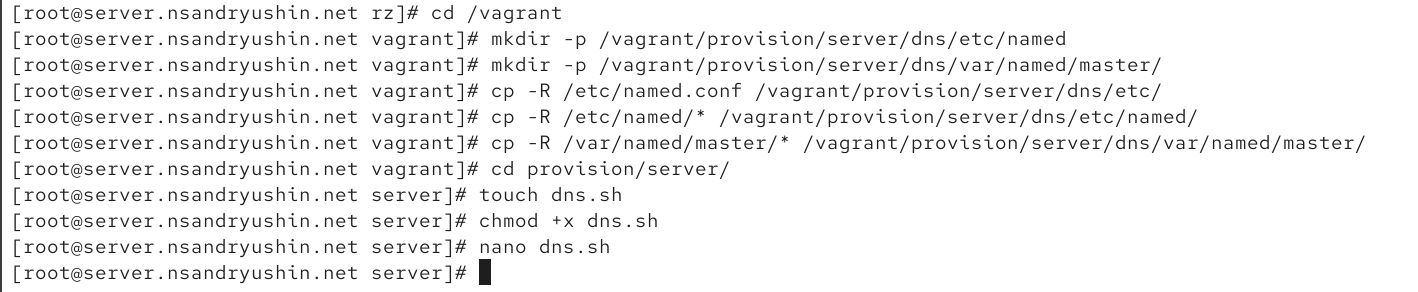
\includegraphics[keepaspectratio]{image/20.png}}

}

\caption{Конфиг вагрант}

\end{figure}%
\end{frame}

\begin{frame}{1.23 скрипт}
\phantomsection\label{ux441ux43aux440ux438ux43fux442}
И напишем скрипт для загрузки вагранта

\begin{figure}[H]

{\centering \pandocbounded{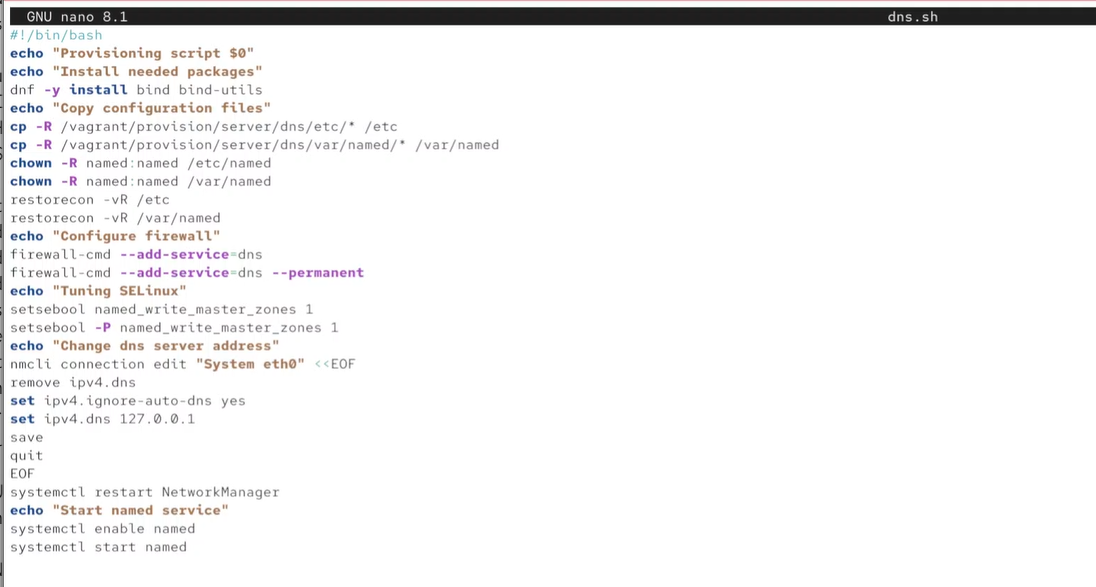
\includegraphics[keepaspectratio]{image/21.png}}

}

\caption{скрипт}

\end{figure}%
\end{frame}

\begin{frame}{1.24 vagrantfile}
\phantomsection\label{vagrantfile}
И в vagrantfile будем загружать этот скрипт

\begin{figure}[H]

{\centering \pandocbounded{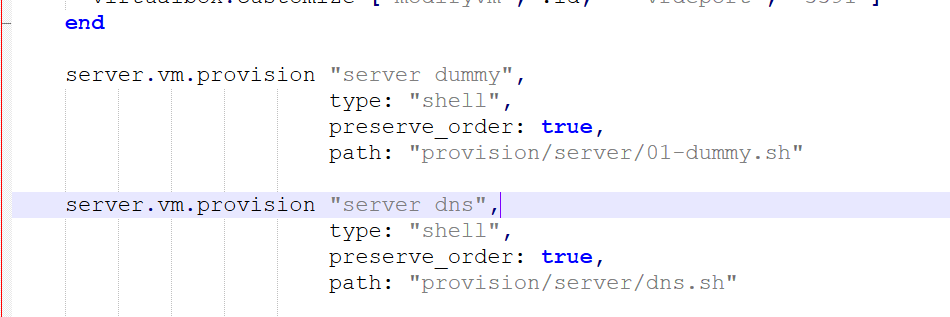
\includegraphics[keepaspectratio]{image/22.png}}

}

\caption{vagrantfile}

\end{figure}%
\end{frame}

\begin{frame}{1.25 Выводы}
\phantomsection\label{ux432ux44bux432ux43eux434ux44b}
В результате выполнения работы были получены навыки настройки днс
\end{frame}




\end{document}
